% !TeX root = ../main.tex
% Add the above to each chapter to make compiling the PDF easier in some editors.

\chapter{Results}\label{chapter:results}

As explained in the previous chapter, this thesis follows several topic modeling approaches to 
obtain the most representative result that can be analyzed. To emphasize the approaches again, 
the first approach follows Martin's general recommendations and does not change any arguments. 
This BERTopic approach delivers around 7500 topics, which is too much to analyze and make sense 
of the results. 

The main reason behind the mass number of topics is \texttt{min\_cluster\_size} remaining at 20, 
allowing around five thousand topics with less than five thousand tweets. The other main reason 
is the diversity of the analyzed data. To determine the topics, sample data of 1\% of all collected 
tweets is used from a dataset that contains more than 200,000 daily tweets. 
When manually looking at the data, one can realize that even though the size is small, the topic 
can be related to a real-life event. Nevertheless, on the other hand, most of the topics can be 
combined or be in the outlier category.

With the experiences from the first approach, the second approach tries to minimize the 
cluster size of the topics to obtain a better result. When the \texttt{min\_cluster\_size} remained 
at 100, around 1000 topics were returned from the topic model. Similar to the first approach, 
this approach also covered the most significant topics. Because the cluster sizes are bigger 
with this approach, the topics are more challenging to label and categorize in one area. Although 
one can realize the similarities between these approaches in the top eight representative words, 
the representative tweets differ. These representative tweets are used in OpenAI prompt to label 
the topics, so the quality of these tweets is of high importance. In this approach, most 
representative tweets include three similar long texts with a high proportion of hashtags and 
mentions. That is also why almost half of the top 20 topics are demands or requests from the 
government, where many users and bots spam almost similar tweets to put the topic in trends, 
promoting politicians, parties, and specific agendas \parencite{secim2023}.
% add additional information here about bots and etc 

After considering these arguments, this thesis mainly analyzes the results of the first approach, 
where one can realize topic trends consisting of specific topics that make comparing and analyzing 
the results considerably more straightforward.

It is essential to mention that outliers are not mentioned via graphs but are remembered 
during the results. Although some approaches in this tried to redistribute outliers, outliers 
exist for a reason. As Grootendorst notes, outliers are to be expected, and pushing the 
output to have no outliers may not correctly represent the data. 

One disadvantage of following the default pipeline of BERTopic is that when the model is first trained, 
the biggest cluster is usually the outliers. However, when training the model and transforming 
the rest of the data, the outlier cluster is considered a usual topic cluster like any other. 
For instance, during one of the approaches, the model had more tweets in the outlier cluster 
while training than after transforming all the collected data, which might, on the one hand, 
cause lots of meaningless topics and, on the other hand, not accurately represent the data. 
There are several new approaches that BERTopic supports that overcome that issue. 
One can try \textit{Online Topic Modeling} to incrementally train the model, or 
\textit{Merge Multiple Fitted Models} approach, where multiple models are trained and, in the end, 
merged so that no information is lost. These approaches are discussed in~\autoref{section:future_work}.
% 

The top results of the topic modeling are presented in \autoref{tab:topic_modeling_results_1}, 
ordered by the number of tweets in the clusters. The \autoref{tab:topic_modeling_results_1} shows 
the topic labels on the left and their respective topic's eight representative words on the right. 
Although it would be hard to translate the representative words, the labels are labeled and then 
translated by GPT-4 Turbo for better interpretation. One can look at the GitHub repository\footnote{\url{https://github.com/EfeSenerr/Thesis_paper}} 
for the original results of the model for the top 50 topics. Since OpenAI models are not cost-free, 
they have been only used for the top 50 topics.

The top 15 topics represent various themes around Turkish political discourse. These topics include 
general political discussions, praise and criticism of both ruling and opposition parties, 
wishes and demands from the government, and the earthquake disaster. 

\begin{table}[h!] % second approach without outleirs
    \centering
    \small
    \begin{tabular}{|>{\hspace{0pt}}m{0.35\linewidth}|>{\hspace{0pt}}m{0.55\linewidth}|} 
    \hline
    \normalsize{\textbf{Topic Label}}                                 & \normalsize{\textbf{Representative Words}}                                                                                                                \\ 
    \hline\hline
    Political Discussions	& \footnotesize{aysedogan1955, yirmiucderece, hassa61, furkancerkes, secimtr2023, cenginyurt52, aykiricomtr, pusholder} \\
    Opposition Candidates 	& \footnotesize{oy, kılıçdaroğlu, oyları, seçmeni, oylar, vermem, aday, seçimde} \\
    Erdoğan \& Nationalism 	& \footnotesize{türk, turkey, türkiye, yüzyılı, türkiyeyüzyılı, stanbul, milliyetçisi, cumhuriyeti} \\
    Religious Wishes	& \footnotesize{allah, versin, eylesin, müslüman, razı, mekanı, namaz, dini} \\
    Political Discussions \& Criticisms	& \footnotesize{cır, terketmek, denilince, uyruklu, ayrilmis, muharremin, vezir\_yuce, bahtiyar\_ergn} \\
    Criticism of Political Figures 	& \footnotesize{siyaset, siyasetin, siyasetiniz, siyasetçi, siyaseti, batsın, siyasete, siyasette} \\
    Opposition Coalition \& Criticism	& \footnotesize{erbakancayazan, örneğinde, yolunuzdan, iddialar, atıldılar, seçicez, ihtimalde, omurgasızlıktır} \\
    Treason Accusations	& \footnotesize{ülkeyi, ülkeye, ülke, ülkenin, ülkede, yağdanlıkları, unutturacaksınız, sığınmayın} \\
    Opposition Figures \& Preferences  & \footnotesize{eu, me, que, aq, pra, amk, tudo, dedem} \\
    Retirement System	& \footnotesize{emeklilik, kısmi, kademeli, emekli, emeklilikte, prim, 5000} \\
    Earthquake \& Demands	& \footnotesize{neticesiz, uzunca, deprem, depremin, süredir, atanma, yumuşak, depremde} \\
    Provocation \& Discussions	& \footnotesize{kızmaz, ahhh, vura, yanarız, soğancı, mitink, arsibjk1903bjk, baskan} \\
    Praise of Political Figures	& \footnotesize{başkanım, başkan, başbakan, başkanın, cumhurbaşkanım, selo, mehmetfatihser5, mehmetersoy57} \\
    Teachers \& Demands	& \footnotesize{öğretmen, öğretmenler, ataması, ilave, ücretli, öğretmenlere, cumhuriyetimizin, öğretmenlerin} \\
    Erdoğan's Election Chance	& \footnotesize{rdoğana, erdoğan, erdoğanı, egemenlere, turda, tura, vereceğim, oyumu} \\
    \hline
    \end{tabular}
    \caption[Overview of Topic Modeling Results with Labels and Representative Words]
    {This table outlines topic modeling results after outlier redistribution, showcasing 
    the top eight representative words per topic via the MMR model, with topic labels generated 
    by GPT-4 Turbo, and manually shortened.}\label{tab:topic_modeling_results_1}
\end{table}

Before diving deeply into the topics and understanding the big picture, clarifying some topics 
for better context would be beneficial. Topics like \textit{Political Discussions}, 
\textit{Political Discussions \& Critism}, \textit{Critism of Political Figures}, 
\textit{Praise of Political Figures} are more general and include tweets with positive and 
negative sentiments towards both the ruling and the opposition parties. 
One can realize that the representative words of the first topic include Twitter user names, 
which are active accounts that share news mainly about the elections. A high number of replies 
and a high level of interaction with their tweets made this category the most noteworthy.

However, topics like \textit{Opposition Candidates}, \textit{Opposition Coalition \& Criticism}, 
\textit{Opposition Figures \& Preferences} and \textit{Erdoğan's Election Chance} focus on and 
express opinions about specific target groups, either the ruling party or the opposition parties 
and their candidates. 

It is hard not to notice the fourth biggest cluster \textit{Religious Wishes}, which includes 
tweets that cover aspects of prayer and Islam. While most of the representative sentences show 
tweets expressing condolences to various political figures who have lost their relatives, many 
of these tweets also include phrases of support and sympathy, such as \textit{'God bless you'}, 
underlining solidarity.

The label \textit{Treason Accusations} might sound absurd. The main reason for that is, again, 
the representative tweets that include some accusations against the political figures, 
blaming them with extremes like committing treason or being a terrorist. As one of the largest 
clusters, topics like this illustrate the polarization within the Turkish political landscape, 
which has been prominent over the years \parencite{cevik_turkey_polarization_2018}. 
Another topic in this table, \textit{Provocation \& Discussions}, also highlights the 
polarization level in the Turkish Twitter political discourse. The representative tweets are 
aggressive and show a high level of emotions.

\textit{Erdoğan \& Nationalism} topic and its representative words show a significant degree 
of nationalist ideas. The label itself includes Erdoğan because of the representative tweets 
mentioning Erdoğan and the tenth representative word \textit{Erdoğan}, which is not seen in the table. 
However, it is essential to mention that both the opposition and ruling party coalition 
include parties based on Turkish nationalism that played a significant role in May 2023 
elections, parties being \ac{IyiP} and \ac{MHP}.

Although it is more explicit in other topic modeling strategies that this thesis tried, 
one can also see the volume of topics like \textit{Teachers \& Demands} and \textit{Earthquake \& Demands} 
in \autoref{tab:topic_modeling_results_1}. The role of Twitter in the latter topic is crucial. 
Because of the earthquake on 6 February, all controversial telecommunication lines were disrupted, 
where Twitter has been widely used for rescue operations \parencite{cevik_aksoy_turkey_earthquake_2023}.

All these mentioned topics are deeply analyzed in the following section, with 
graphs supporting understanding of the topics and their trends.

\section{Detailed Analysis of Topic Categories}

For simplicity and better understanding purposes, this thesis analyzes the topic modeling results 
in three categories: topics related to the ruling party visualized in \autoref{fig:topics_graph_akp}, 
the opposition visualized in \autoref{fig:topics_graph_opposition}, and the remaining topics 
visualized in \autoref{fig:topics_graph_other}. 

These graphs visualize the selected topics in a normalized monthly distribution. 
Normalization has been done considering the top 50 topics. Otherwise, the interpretation of topics 
and their trends was almost impossible. One can not realize any trends in a frequency graph because 
the \#Secim2023 dataset is not collected equally between months, demonstrated in \autoref{fig:collected_tweets}.

In all these graphs, the biggest cluster \textit{Political Discussions} is shown as the baseline 
in a straight blue line to compare these different graphs and analyze the trends more smoothly. 

\subsection{Ruling Party Discourse Analysis}

\begin{figure}[htb]
    \centering
    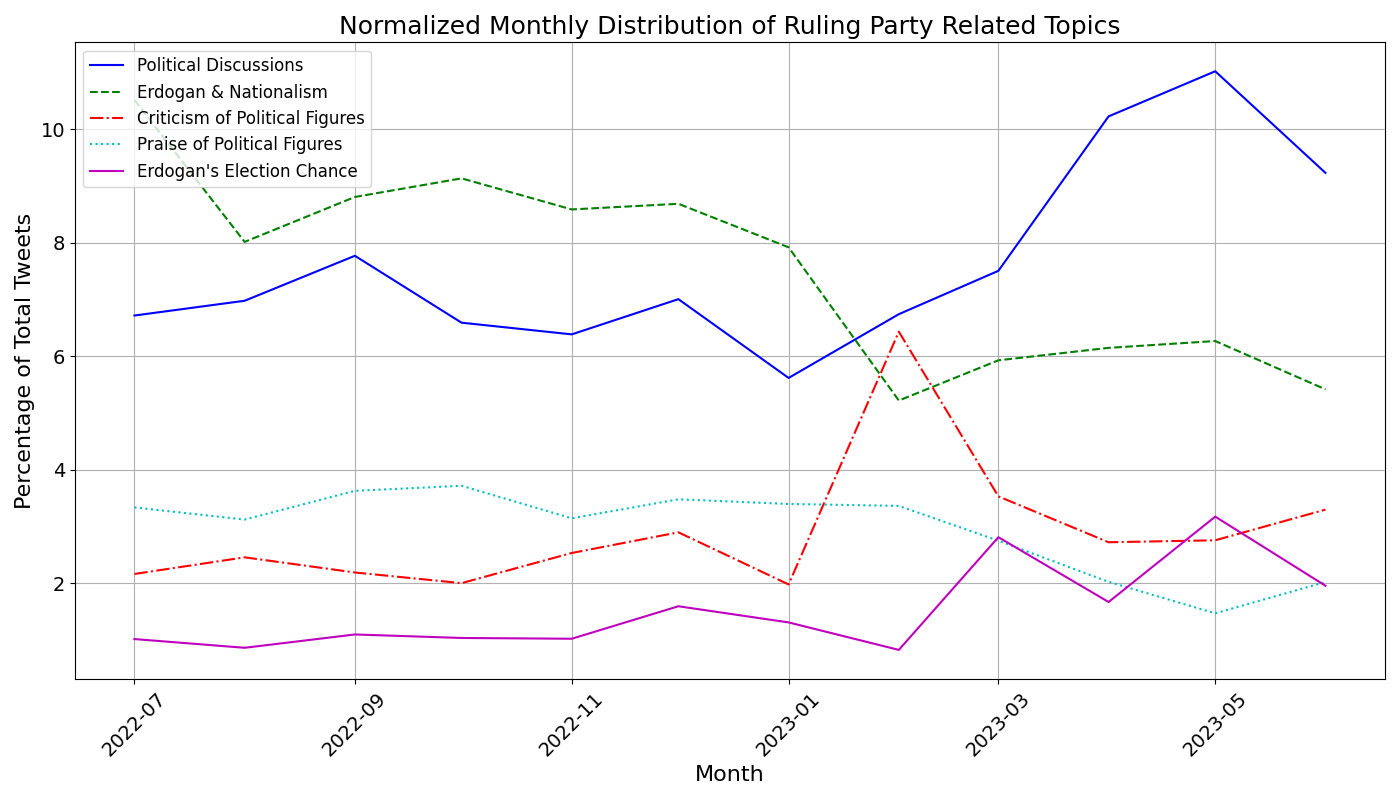
\includegraphics[width=\linewidth]{figures/normalized_akp_selected_topics_distribution_with_styles.png}
    \caption[Normalized Monthly Distribution of Ruling Party Related Topics]
    {This figure shows the proportion of ruling party-related topics among the top 50 topics. 
    The blue line represents the biggest cluster as the baseline, while other lines represent topics 
    related to Erdoğan and the ruling party.}\label{fig:topics_graph_akp}
\end{figure}

Beginning the analysis with the first graph~\ref{fig:topics_graph_akp}, 
it covers the monthly distribution of the ruling party and Erdoğan-related topics. 
It is essential to acknowledge the baseline topic \textit{Political Discussions}, 
keeping its importance in the months to elections, massively increasing after the start of 2023 up 
to more than 10\% of the top 50 tweets. That is normal, considering that in the months leading up 
to the elections, almost all the news was political, and rallies around Turkey were happening daily. 
Undecided opposition candidacy, hot topics like the economic crisis and migration policy, and 
uncertainties in domestic and foreign policies led social media to a political discussion hub.

Having the baseline topic covered, the next topic with a green dotted line covers the topic 
\textit{Erdoğan \& Nationalism}. As mentioned previously, it is essential not to converge Turkish 
Nationalist ideas with Erdoğan and the AKP regime. There are nationalism-based parties in both the 
opposition and the ruling coalition. The opposition coalition's name is even `Nation Alliance', 
in other words, the `Table of Six'.

Turkish Nationalism has always been one of the base ideas of Turkish politics since the republic's 
foundation. The reason for that is now the opposition and once the founding party, \ac{CHP}, who laid 
Turkey's six founding fundamental ideologies called the `Six Arrows'. 
One of the \textit{arrows} represents Nationalism. However, as Hotelling's model suggests, 
throughout the years, because CHP's idealogy moved more toward the left wing, parties like AKP or 
newly established parties like ZP started to fill the empty right-wing spots \parencite{caramani_comparative_politics_2020}. 
Representative tweets showing support for different political figures using nationalist 
ideas also underline this aspect. 

The migration policy was one of the hottest topics of the May 2023 elections. 
The government's attitude of welcoming more than six million refugees while getting funding from the 
European Union for this purpose sparked lots of tensions amongst different ideologies and parties. 
In 2021, a new party called the \ac{ZP} was formed from the ranks of the opposition. 
It then rapidly increased its popularity as a mainly single-issue party focused on expelling refugees 
back to their countries \parencite{berk_esen_turkish_politics_2023}. \ac{ZP} formed the second opposition 
coalition against Erdoğan, and their candidate received more than 5\% of the votes. 

These events highlight why Nationalism has been one of the most trending topics during the months up 
to the election. However, in the new year, more specifically after the 6 February earthquake, other 
topics gained more significance, which can also be seen in the \autoref{fig:topics_graph_akp}.

One of the topics that gained relatively more importance is the \textit{Criticism of Political Figures}, 
visualized as a red dotted and straight line in \autoref{fig:topics_graph_akp}. On the other hand, 
the topic \textit{Praise of Political Figures}, visualized as a turquoise dotted line, has lost volume 
in time. The main explanation for that is the 6 February earthquake, which immediately changed 
the course of the elections by changing everybody's attention towards the southeast of Turkey. 

The following reasons, also underlined by \textcite{cevik_aksoy_turkey_earthquake_2023}, can explain 
the change in the trends of these topics, where criticism outweighed the praise of political figures 
on Twitter. The system lacked law enforcement until the earthquake, where the 
contractors of the building constructions sought to maximize their profits without taking the 
necessary precautions. 
The weakened state capacity led to the slowness of emergency response during the catastrophe. 
The military was missing, and there were no plans against this kind of emergency, or in other words, 
if there was a plan, it was not executed thoroughly. 
NGOs and volunteers organized themselves and worked together for days after the earthquake. Twitter was always 
the central platform for organizations and cry for help. Nonetheless, the government slowed down 
Twitter to prevent `disinformation' from spreading, which worsened this process.

The last topic in this graph is \textit{Erdoğan's Election Chance}, visualized as a pink straight line. 
It can be seen that this topic remained relatively low and reached the bottom rock during the month 
of the earthquake, and in March, it increased a lot and outranked the other two topics in the election 
month. The reasons for this increase will be discussed thoroughly in \autoref{fig:topics_graph_opposition}. 
However, in short, the lack of collaboration and not being decisive about a candidate among the 
opposition ranks make this increase feasible. Polls also support this 
argument \parencite{cevik_aksoy_turkey_earthquake_2023}.

\subsection{Opposition Discourse Analysis}

\begin{figure}[htb]
    \centering
    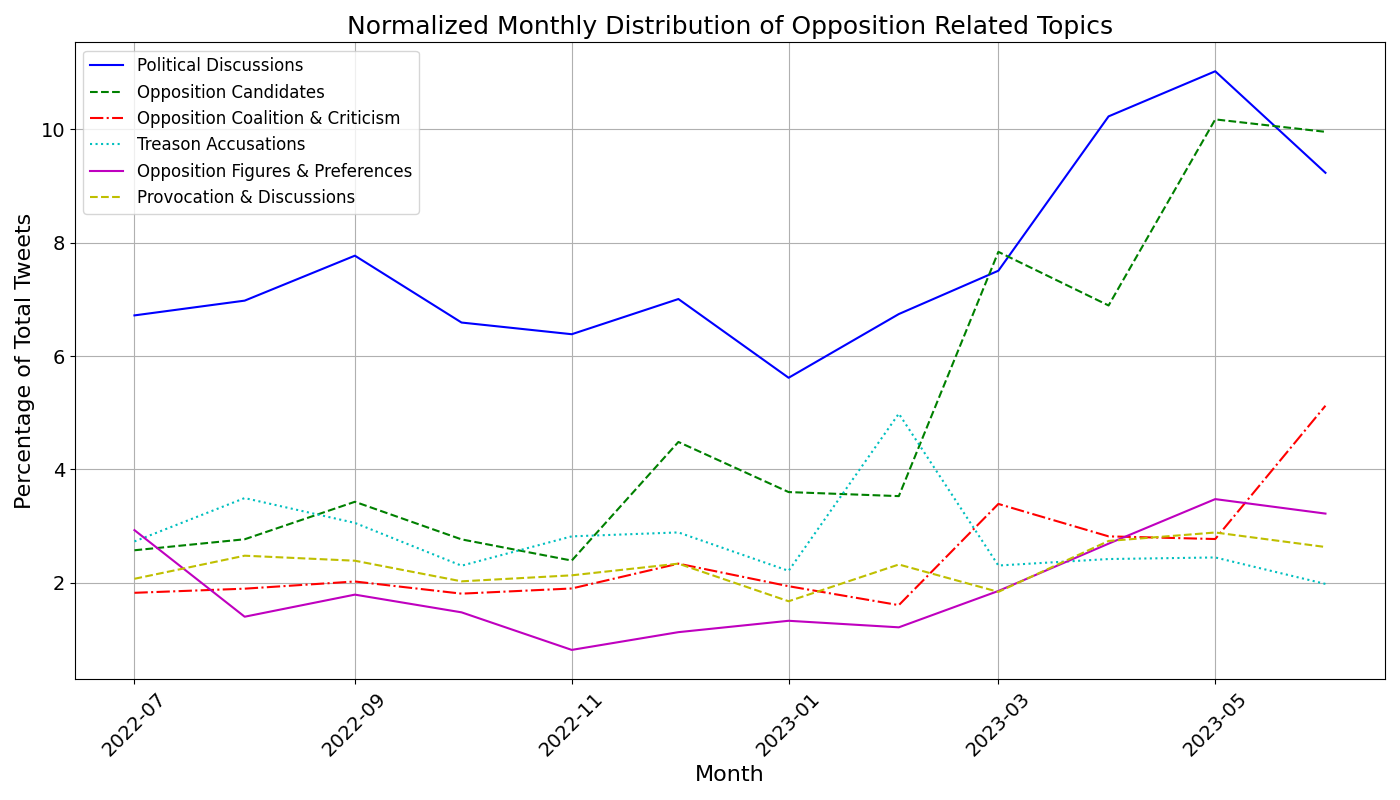
\includegraphics[width=\linewidth]{figures/normalized_opposition_selected_topics_distribution_with_styles.png}
    \caption[Normalized Monthly Distribution of Opposition Related Topics]
    {This figure shows the proportion of opposition-related topics among the top 50 topics. 
    The blue line represents the biggest cluster as the baseline, while other lines represent topics 
    related to opposition parties and their candidates.}\label{fig:topics_graph_opposition}
\end{figure}

The analysis continues with the other side of the table, \autoref{fig:topics_graph_opposition}, 
which covers the monthly distribution of the opposition-related topics. As a reminder, 
\textit{Political Discussions} topic can also be found in this graph, which is used as a baseline 
for comparing the graphs.

Continuing with the second topic, \textit{Opposition Candidates} visualized as a green line in the 
graph. While the representative words cover topics like vote, the main opposition coalition 
Nation Alliance's candidate Kılıçdaroğlu, and elections, the representative tweets are about 
people's opinions about who they would vote for in the opposition ranks. For instance, some of 
them state that \textit{'they would not vote for Kılıçdaroğlu, who does not have any victory 
against Erdoğan for all these years.'}, or  \textit{'they would only vote for Mansur Yavaş'}, 
who is the mayor of the capital city Ankara. 

It is essential to present some context here. The main opposition coalition, Nation Alliance, 
a.k.a. `Table of Six', consists of six parties that signed a joint manifesto in 2022 outlining 
plans to abolish the presidential system and restore the rule of law and civil liberties by 
returning to the previous parliamentary system \parencite{berk_esen_opposition_alliance_2023}. 
The coalition wanted to achieve this goal by selecting a joint presidential candidate. 
Like most people in the opposition ranks, \parencite{berk_esen_opposition_alliance_2023} saw 
selecting a joint presidential candidate as the most demanding task. 
Since the president holds immense powers in the Turkish presidential election system, the parties 
were uncertain whether to hand that authority to one individual, so they sought to concentrate 
more on the alliance than the candidate. Due to these reasons, the coalition pushed this matter 
further back and could only start to discuss these matters after the earthquake, which is easily 
remarkable on \autoref{fig:topics_graph_opposition}. 

In March 2023, the majority of parties in the coalition then agreed on Kılıçdaroğlu, 
who was the leader of the main opposition party \ac{CHP} and also played an essential role in 
the establishment of this coalition. 
After the agreement, the second largest opposition party \ac{IyiP} also considered that although 
Kılıçdaroğlu's collaborative personality and focus on unity was an asset for a democratic 
transition, but stood behind the idea that this could weaken his electoral prospects against 
Erdo­ğan. As noteworthy evidence, one could show the most recent polls showing that he 
follows the popular mayors of Ankara, Mansur Yavaş; Istanbul, Ekrem Imamoğlu, and even the 
\ac{IyiP} leader Meral Akşener \parencite{berk_esen_opposition_alliance_2023}.

The trending level of the topic also aligns with the social movements at that time 
\parencite{gultekin_kilicdaroglu_aday_2023}. 
Just before the earthquake, on 5 February, Kılıçdaroğlu's candidacy topic sparked again. 
There were campaigns against Kılıçdaroğlu on the streets and also on social media with a slogan 
\textit{'Do not be a candidate Kılıçdaroğlu.'}. People were holding pan cards with the same slogan 
in front of the \ac{CHP} general headquarters and sharing it on Twitter \parencite{ulas_kilicdaroglu_aday_pankart_2023}. 
Some influencers even planned to march to the headquarters the next day to prevent his candidacy. 
That is one of the main reasons why the earthquake on 6 February changed and deeply affected 
the discourse of the May 2023 elections.

\ac{IyiP} considered Kılıçdaroğlu lacked sufficient public appeal to win the elections. 
That is why Akşener opposed his candidacy and supported the mayors of Ankara and Istanbul. 
In short, after several days, the parties agreed on the vice presidency of these two mayors and 
continued the election campaign as a united front. All these events resulted in the topic 
\textit{Opposition Candidates} naming itself as the most articulated topic in March on Twitter, 
surpassing the baseline. Even after the election month, the topic continued to be relevant, 
beating the baseline again. The discussion rallied then around whether Kılıçdaroğlu was 
\textit{'the right candidate'}. Several months after the elections, Kılıçdaroğlu lost the in-party 
elections after leading the main opposition party for 13 years \parencite{gundogan_chp_özgür_özel_2023}.

%\%35 oy orani (?)

The next trending topic, \textit{Opposition Coalition \& Criticism} visualized as a red straight 
and dotted line, follows a similar tendency, gaining importance in March and continuing to 
grow even after the elections. However, this topic mainly focuses on direct criticism against 
the opposition parties. For example, the representative tweets in this cluster complain about 
Ali Babacan, the leader of \ac{DEVA}, called him a puppet whose' congressman candidates were 
entering the elections in the same list as \ac{CHP}. On the other hand, some tweets refer to 
Kılıçdaroğlu as a traitor to his own party for this very same reason.

The following topic, \textit{Treason Accusations} visualized as a turquoise dotted line, shows 
accusations against those who did not support the same idealogy as the writer of these Tweets. 
Blaming political figures with extremes like committing treason or being a terrorist is a standard 
tongue that brings the polarization in the Turkish political discourse to light. 
One can observe that this topic gained importance in February. 
The reason can be easily tied to the earthquake, such as people accusing the government of lacking 
law enforcement or not taking the necessary measures for the earthquake.

Represented as a pink straight line, \textit{Opposition Figures \& Preferences} highlights a mixture of 
tweets that include swear words, foreign words and sentences, and discussions around opposition figures.
One can understand the abbreviations of Turkish swearwords in the representative words column in 
\autoref{fig:topics_graph_opposition}, and it is likely that the BERTopic topic model could not make any 
sense of the words and merged the topic with foreign words and sentences. 
Another point the topic model had difficulties understanding is the word \textit{'dedem'}, 
translated to \textit{'my grandfather'}. Grandfather nickname has been used by the younger generation on 
social media and overall to refer to the opposition candidate Kılıçdaroğlu. The nickname itself has more of a 
positive sentiment, emphasizing his kindness and, on the other hand, his age. 
Although this topic beat all other topics than the baseline topic in July 2022, it started to gain importance 
when the elections were getting closer and peaked during election month, possibly related to unexpected 
election results, including comments about the opposition.

The topic, \textit{Provocation \& Discussions}, marked by a yellow dotted line, indicates the polarization 
level in the Turkish Twitter political discourse, as stated before. The representative tweets are aggressive 
and show negative sentiments, with some of the tweets accusing political figures of being provocateurs. 
The trend of the topic continues steadily, increasing slightly just before the election month.

\subsection{Other Relevant Discourse Analysis}

\begin{figure}[htb]
    \centering
    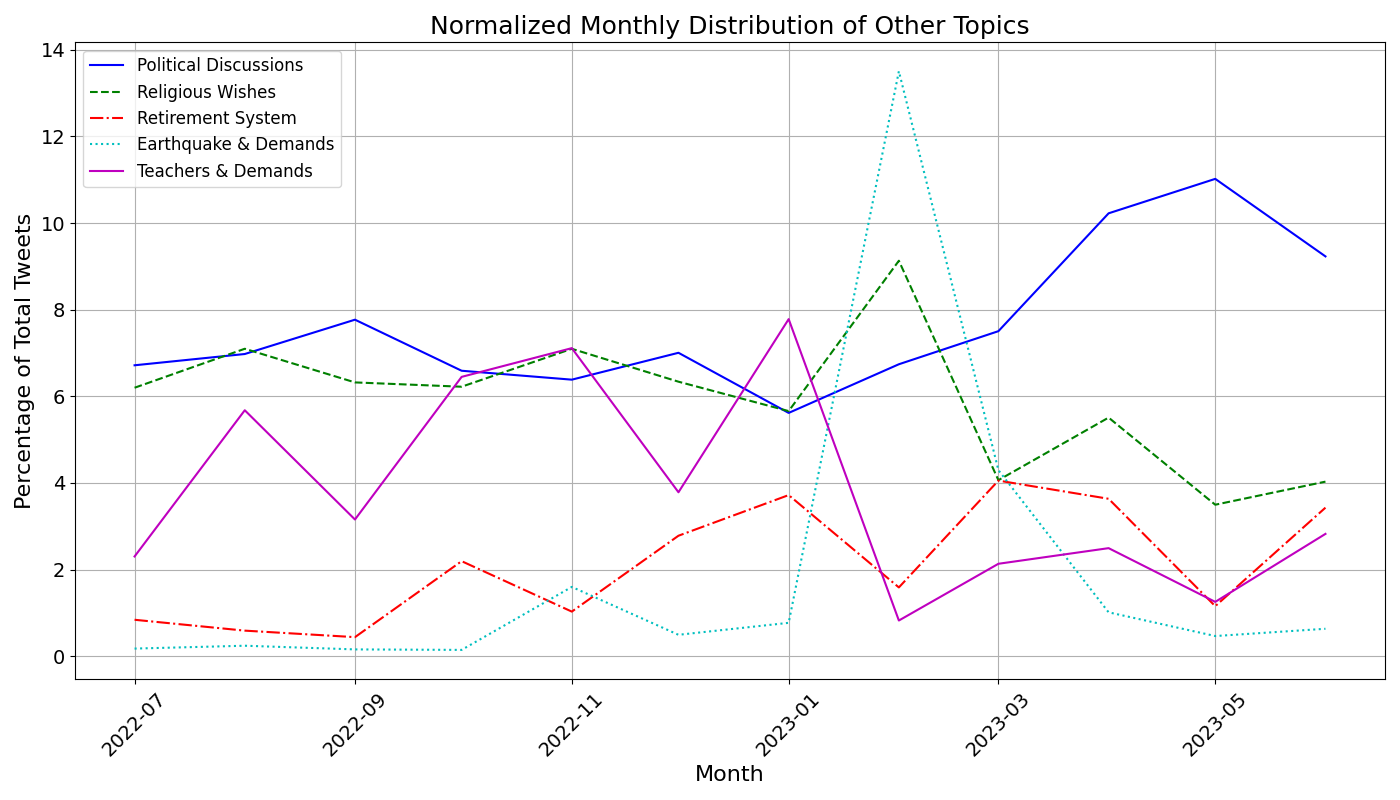
\includegraphics[width=\linewidth]{figures/normalized_other_selected_topics_distribution_with_styles.png}
    \caption[Normalized Monthly Distribution of Other Topics]
    {This figure shows the proportion of opposition-related topics among the top 50 topics. 
    The blue line represents the biggest cluster as the baseline, while other lines represent topics 
    like demands from the government and the earthquake.}\label{fig:topics_graph_other}
\end{figure}

The analysis proceeds with the last graph, as presented in \autoref{fig:topics_graph_other}, showcasing the 
monthly trends of other than ruling party or opposition-related topics. As the baseline, 
\textit{Political Discussions} topic can be seen as the blue straight line in the graph. 
One can realize that multiple topics have crossed the baseline topic over the months up to the election. 

Kicking things off with the topic \textit{Religious Wishes}, visualized as a green line, the topic contains 
tweets that cover aspects of prayer and Islam. It features representative words like \textit{'Allah'}, 
\textit{'müslüman'}, and \textit{'din'}, which than translates to \textit{'Muslim'} and \textit{'religion'}. 
Some representative sentences exhibit tweets praising political figures from different ranks, 
saying \textit{'God bless you'}. 
Although the topic remained at the same level as the baseline and peaked during the month of the earthquake, 
afterward, it kept its importance while falling in volume, leaving room for political discussions.

Illustrated with a red straight and dotted line, the \textit{Retirement System} topic demonstrates tweets 
around the retirement system policies. Before the elections, one of the government's promises was to renew 
the last social security legislation in 1999. At the beginning of March, the government passed new legislation 
that softens existing rules on retirement age and retirement eligibility requirements, allowing almost more 
than 2 million workers to retire immediately \parencite{erdem_bisgin_retirement_2023}. 

With the enactment of new legislation and a massive increase in the minimum wage, the government increased its 
spending massively, which resulted in increased public opinion just before the elections 
\parencite{cevik_aksoy_turkey_earthquake_2023}. One can recognize that the topic peaked in the month of 
enactment, slightly lowering in volume afterward.

The topic \textit{Earthquake \& Demands} is self-explanatory, highlighting the earthquake on 6 February. 
In the earthquake, more than 53,000 people lost their lives, which created a social trauma and changed the 
course of the elections. Although the government mishandled the earthquake, as 
\textcite{cevik_aksoy_aydin_turkey_after_elections_2023} shares, the opposition failed to get the votes 
from the region, and Erdoğan maintained his popularity in the region, where he received more than 
70\% the votes in some provinces \parencite{michaelson_narli_earthquake_regions_erdogan_2023}.
As mentioned previously, the role of social media in the earthquake is noteworthy.
It is remarkable that the topic peaks massively in February. However, it is very interesting, and maybe 
also not expected, that it lost almost all of its volume in just two months, making just around 
1\% of the tweets afterward. 

The last topic in the examination is \textit{Teachers \& Demands}. The representative sentences exist 
of sentences like \textit{'We demand 100 thousand additional teacher positions.'}. One of the 
representative words \textit{'cumhuriyet'}, translated to \textit{'republic'}, points out that tweets 
exist of a rhyme, calling for an additional 100 thousand teachers at the 100.\ anniversary of the Turkish 
Republic. The massive volume of this topic can not be unseen, almost beating the baseline topic two times. 
It is essential to mention that, as \textcite{pfeffer_twitter_24_Hours_just_another_day_2023} also points 
out, Twitter has been used through bots and different means of coordinated automated activities to show 
influence and power in the public discourse by making the relevant topic trending and keeping it before eyes.

Regardless, this topic aligns with the agenda of the Nation Alliance, where the coalition promised to 
create new positions for the teachers in one of their rallies \parencite{trt_ogretmen_atamasi_kk_2023}.

% research questions partly addressed: 
% - "in what ways do these shifts mirror political movements?"

\section{Supplementary Visual Insights}

This chapter presents additional visual representations of the topic model results.  

The first visualization is inspired by Maarten Grootendorst, who visualized the topic model 
results from millions of Wikipedia pages in his Huggingface 
repository\footnote{\url{https://huggingface.co/MaartenGr/BERTopic_Wikipedia}}. Like this thesis, 
he also used BERTopic for big data analysis and visualized the results in the end. 

\begin{figure}[h!]
    \centering
    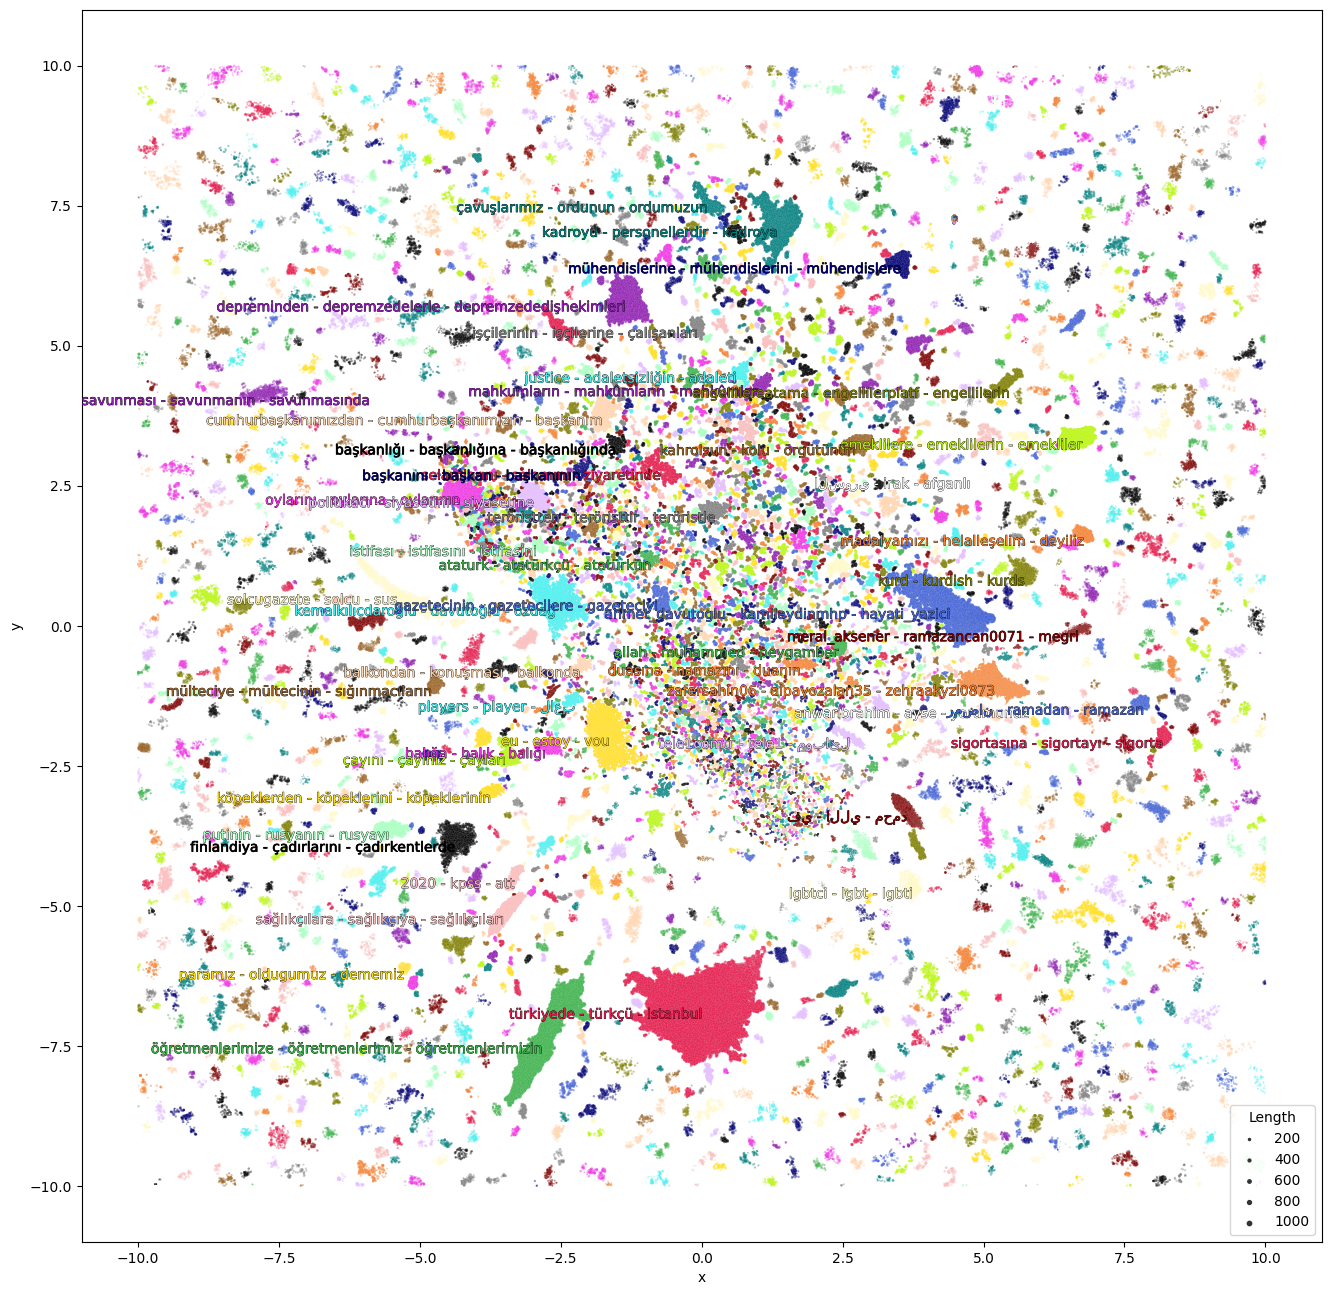
\includegraphics[width=\linewidth]{figures/visualization_2d.png}
    \caption[The Top 50 Topics Visualized in Two-Dimensional Embedding Space Using cuML's UMAP]
    {This visualization presents the top 50 topics reduced to a two-dimensional embedding space using 
    cuML's UMAP, following Maarten Grootendorst's guidelines.\footnotemark}\label{fig:topics_2d}
\end{figure}
\footnotetext{\url{https://huggingface.co/MaartenGr/BERTopic_Wikipedia}}

The \autoref{fig:topics_2d} presents the top 50 topics, which have been reduced to 
two-dimensional embedding space using UMAP.
It pictures different clusters with different colors with respect to their sizes and 
does not contain any outliers. The white background could not be seen if the figure would 
have included outliers. 
The topics are illustrated by their top three representative words. One can realize that 
their top three representative words can differ from the ones from the previous table, 
\autoref{tab:topic_modeling_results_1}. 

This is because a different BERTopic pipeline has been used for this visualization. 
This pipeline includes pre-computing of required parameters of BERTopic, which are generally 
computed during the fitting procedure. Different from the training pipeline of the base topic 
model explained in \autoref{chapter:bertopic_pipeline}, the first step starts with UMAP, 
which has a parameter \texttt{n\_components} of two instead of five. 
That leverages the power of GPU by using the cuML library and reduces the topics to two-dimensional 
space. 

Afterward, HDBSCAN uses the two-dimensional reduced embeddings to pre-compute the clusters of 
the topics from scratch. These results can be fed to BERTopic to perform manual topic 
modeling\footnote{\url{https://maartengr.github.io/BERTopic/getting_started/manual/manual.html}}.
If the model already has topic labels, it can use those to label them using various 
representation models.

With embeddings, reduced dimensionality and clusters on hand allow the speeding up of the fitting 
process. Additionally, Grootendorst presents a trick to get better results. 
He states that if one directly gives BERTopic the reduced embeddings, BERTopic would use those 
to create topic vectors, which could be better. For better results, he suggests giving the model 
the full embeddings and creating a custom dimensionality reduction class that will return the 
reduced embeddings. Further details can be found in the thesis GitHub repository.

The results of this pipeline are then used for visualizing the \autoref{fig:topics_2d}, 
with the usage of \texttt{seaborn} and \texttt{matplotlib} library.

Some of the topics are relatively straightforward to pick up. The enormous red cluster on the 
bottom of the figure, titled as \textit{'türkiyede -- türkçü -- istanbul'}, visualizes the 
topic GPT-4 Turbo labeled as \textit{Erdoğan \& Nationalism} from the default pipeline. 
Next to that topic to the left, visualized as a green pipeline, is the topic 
\textit{Teachers \& Demands}. 

The middle of this figure is considerably chaotic. Almost all of the clusters in the middle are 
related to the election. The topics from the political figures, votes, major Twitter accounts, 
and the resignation of known figures are covered. At the top of the figure, the cluster 
related to the earthquake can be seen as purple, titled as 
\textit{'depreminden -- depremzedelerle -- depremzede'}.

\begin{figure}[h!]
    \centering
    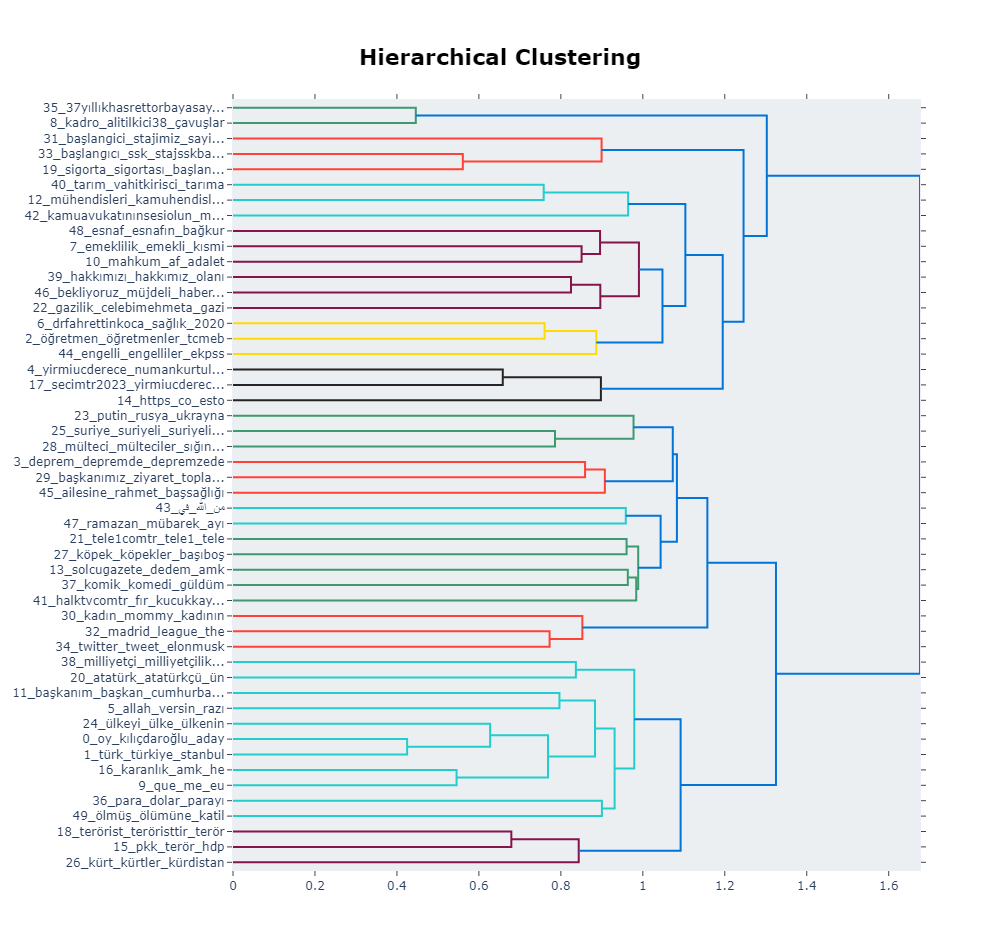
\includegraphics[width=\linewidth]{figures/Hierarchical_Clustering.png}
    \caption[Hierarchical Clustering of the Top 50 Topics]
    {This visualization presents the hierarchical clustering of the top 50 topics 
    using BERTopic functions.}\label{fig:topics_hierarchical_clustering}
\end{figure}

The following visualization, \autoref{fig:topics_hierarchical_clustering}, is about the hierarchical 
clustering of the top 50 topics of the sampled data and has been created using BERTopic 
function \texttt{visualize\_hierarchy()}. The fitted BERTopic model has been used, and the 
parameter \texttt{top\_n\_topics} has been set to 50, which returns that figure. A ward linkage 
function performs the hierarchical clustering based on the cosine distance matrix between topic 
embeddings. Since the GPT-4 Turbo labeling has been done after fitting the model, and only 
for the top 50 topics, the labels in the figure show default labels after the fitting. 
One can look at the English labels of each top 50 topic in the GitHub repository of the thesis.

If the \autoref{fig:topics_hierarchical_clustering} is deeply analyzed, the topics are divided 
into different colors, which are then connected together to build the total representation. 
The colors present 13 main subjects among the top 50 topic representations.

Beginning the exploration with the top topics, the green cluster represents the demands of military 
sergeants willing to be permanently employed. A batch of sergeants who worked on a limited contract
in the state institutions for almost 36 years sought permanent employment.

The subsequent topic, visualized as red, addresses the demands of young people endorsing their 
internships to be recognized as the start date for their insurance, a critical factor determining 
the start of retirement eligibility.

The following three topics, visualized as turquoise, brown, and green, represent the concerns of 
agriculture engineers and their work appointments, the retirement system, teachers, and their 
demands, respectively. The last topic in the top cluster covers general political discussions on 
Twitter.

Commencing with the bottom cluster, the green cluster illustrates topics related to foreigners, 
refugees, and specifically, people from Ukraine and Syria in separate subclusters. 
The volume of the topic related to Ukraine has stayed at a high level since the beginning of the 
dataset till the beginning of 2023, and the importance of the migration policy in the May 2023 
elections was discussed in the previous section. 

The succeeding two topic clusters, visualized as red and turquoise, demonstrate topics related to 
the earthquake, Arabic texts and Ramadan, respectively. 

The next two clusters, colored as green and red, contain eight different partially political 
topics that are challenging to generalize. One topic that is considerably interesting to point 
out would be the topic titled as \textit{27\_köpek\_köpekler\_başıboş}. It refers to problems 
caused by free-roaming dogs on the streets of Turkey, including increased dog attacks, hygiene 
concerns, safety risks, and traffic accidents, worsened by uncontrolled abandonment and the 
expansion of these animals in public spaces. 

Another topic to highlight is the topic with \textit{30\_kadın\_mommy\_kadının}. \textit{kadın} 
can be translated to \textit{woman} and both \textit{kadın} and \textit{mommy} refers to the 
\ac{IyiP} leader Meral Akşener. Most of the young people on Twitter refer to her as a mom, 
underlining her warmth and sympathy.

The topic titled as \textit{34\_twitter\_tweet\_elonmusk} contains representative words 
referring to Elon Musk's acquisition of Twitter, which started around April and concluded 
around Oktober, the timeframe which this dataset also partially covers.

The second last cluster, portrayed as turquoise, covers various political topics from Nationalism 
to Atatürk, from political figures to presential candidates, from religious wishes to treason 
accusations, from exchange rates to other economic topics. 

The last cluster, illustrated as brown, covers topics related to terrorism and the 
Kurdish community. One can realize the topic titled as \textit{15\_pkk\_terör\_hdp}, which includes 
in its top three representative words terrorism and \ac{HDP}. \ac{HDP} received around 9\% of 
the votes in the May 2023 elections, with a significant portion of their support coming 
from the Kurdish community. The AKP government and other nationalists accuse HDP that it is 
linked to the banned \ac{PKK}, which the European Union also lists as a ter­ror­ist organization 
\parencite{berk_esen_opposition_alliance_2023}, which we can also see from the topic representation
being in the top 50 topics and its' representative tweets.

To remind it again, the extensive Turkish results and graphs, including the code, can be found 
on the GitHub repository of the thesis.


% hierarchical topic model figure fig_hieararchy_50.html: 
% the top part represents requests from the government
% and the bottom part represents other topics

% add table of topics, keywords, openai labels
% add english/turkish one at the end of the thesis

% BELOW ARE TABLES COMMENTED OUT

% \begin{table}[htpb]
%     \centering
%     \begin{tabular}{|c c c|} 
%      \hline
%      \textbf{Topic} & \textbf{Count} & \textbf{Label} \\ [0.5ex] 
%      \hline\hline
%      1 & 4711805 & Elections, Candidates, and Political Discussions \\
%      2 & 2781739 & Erdogan and Political Developments \\
%      3 & 2704097 & Political Agenda and Demands \\
%      4 & 1561746 & Religious Wishes and Political Figures \\
%      5 & 1302418 & Teacher Appointments and Their Demands \\
%      6 & 1286107 & Earthquake and Relevant Requests \\
%      7 & 1222694 & Nation and Country \\
%      8 & 1049210 & Leading Figures in Turkish Politics \\
%      9 & 1022569 & Fair Trial and General Amnesty Requests \\
%      10 & 939330 & Mixed Emotions \\
%      11 & 873148 & Civil Servants and Their Demands \\
%      12 & 833265 & Retirement System and 5000 Premium Partial Retirement \\
%      13 & 813741 & Main Appointment Requests from Reserves \\
%      14 & 766576 & Medical Secretary Appointment Demands \\
%      15 & 759860 & 2023 Turkey Election News and Comments \\
%      16 & 704353 & Internship Grievances and Solution Calls \\
%      17 & 699035 & Staff Sergeant Position Demands \\
%      18 & 667885 & Industrial Internship Victims and Their Rights \\
%      19 & 640073 & Police Training Candidates Interview and Quota Requests \\
%      20 & 627449 & Political Dialogue in Hopes and Expectations \\
%      \hline
%     \end{tabular}
%     \caption[Result of the topic modeling]{Top 20 topics from the result of the topic modeling
%     with their respective topic label and count.}\label{tab:topic_modeling_results}
% \end{table}

% \begin{table}[htpb]
%     \centering
%     \begin{tabular}{|c | c | c|} 
%      \hline
%      \textbf{Topic} & \textbf{Count} & \textbf{Label} \\ [0.5ex] 
%      \hline\hline
%      1 & 4711805 & Seçimler, Adaylar ve Siyasi Tartışmalar \\
%      2 & 2781739 & Erdogan ve Türkiye Siyasi Gelişmeleri \\
%      3 & 2704097 & Türkiye Siyasi Gündem ve Talepler \\
%      4 & 1561746 & Dini Temenniler ve Siyasi Figürler \\
%      5 & 1302418 & Öğretmen Atamaları ve Talepleri \\
%      6 & 1286107 & Deprem Sonrası Yapı Kayıt Talebi \\
%      7 & 1222694 & Ülke ve Millet Konulu Siyasi Tartışma \\
%      8 & 1049210 & Türk Siyasetinde Önde Gelen Figürler \\
%      9 & 1022569 & Adil Yargılama ve Genel Af Talebi \\
%      10 & 939330 & Karışık Duygular ve İletişim Çıkmazı \\
%      11 & 873148 & Kamu Şefleri ve 3600 Ek Gösterge Talebi \\
%      12 & 833265 & EYT ve 5000 Prim Kısmi Emeklilik \\
%      13 & 813741 & Yedeklerin Asıl Atama Talebi \\
%      14 & 766576 & Tıbbi Sekreterlik Atama Talepleri \\
%      15 & 759860 & 2023 Türkiye Seçim Haberleri ve Yorumları \\
%      16 & 704353 & Staj Mağduriyeti ve Çözüm Çağrıları \\
%      17 & 699035 & Uzman Çavuşlar Kadro Talebi \\
%      18 & 667885 & Sanayide Staj Mağdurları ve Hakları \\
%      19 & 640073 & POMEM Adaylarının Mülakat ve Kontenjan Talebi \\
%      20 & 627449 & Umut ve Beklentilerde Siyasi Diyalog \\
%      \hline
%     \end{tabular}
%     \caption[Result of the topic modeling]{Top 20 topics from the result of the topic modeling
%     with their respective topic label and count.}\label{tab:topic_modeling_results3}
% \end{table}

% \begin{table}[htpb]
%     \resizebox{\textwidth}{!}{%
%     \centering
%     \begin{tabular}{|c|c|p{3cm}|p{7.5cm}|} 
%      \hline
%      \textbf{Topic} & \textbf{Count} & \textbf{Label} & \textbf{Representative words} \\ [0.5ex] 
%      \hline\hline
%      1 & 4711805 & Seçimler, Adaylar ve Siyasi Tartışmalar & oy, kılıçdaroğlu, aday, seçim, erdoğan, tayyip, seçimi, istifa, na, turda \\
%      2 & 2781739 & Erdogan ve Türkiye Siyasi Gelişmeleri & türk, türkiye, stanbul, yüzyılı, turkey, türkiyeyüzyılı, ankara, cumhuriyeti, erdogan, milleti \\
%      3 & 2704097 & Türkiye Siyasi Gündem ve Talepler & yirmiucderece, numankurtulmus, aysedogan1955, cenginyurt52, herkesicinchp, meral\_aksener, secimtr2023, hassa61, yildirimkaya40, yilmaztunc \\
%      4 & 1561746 & Dini Temenniler ve Siyasi Figürler & allah, versin, razı, eylesin, müslüman, etsin, din, rabbim, rahmet, cennet \\
%      5 & 1302418 & Öğretmen Atamaları ve Talepleri & öğretmen, öğretmenler, tcmeb, ataması, prof\_mahmutozer, 100, bin, kpss, öğretmenlerin, atama \\
%      6 & 1286107 & Deprem Sonrası Yapı Kayıt Talebi & deprem, depremde, depremzede, depremin, yapıkayıt, yumuşak, depremden, müstakil, planlayanlar, depreme \\
%      7 & 1222694 & Ülke ve Millet Konulu Siyasi Tartışma & ülkeyi, ülke, ülkenin, ülkeye, ülkede, millet, milletin, milleti, millete, senin \\
%      8 & 1049210 & Türk Siyasetinde Önde Gelen Figürler & başkanım, başkan, cumhurbaşkanım, mansuryavas06, ekrem\_imamoglu, başbakan, cumhurbaşkanı, sayın, genel, tanjuozcanchp \\
%      9 & 1022569 & Adil Yargılama ve Genel Af Talebi & mahkum, af, adalet, genelaf, 77, adil, adli, mahkumlar, ihlali, cezalar \\
%      10 & 939330 & Karışık Duygular ve İletişim Çıkmazı & que, me, eu, não, no, dedem, aq, amk, pra, lo \\
%      11 & 873148 & Kamu Şefleri ve 3600 Ek Gösterge Talebi & sırtlayan, hafızası, kurumların, yükünü, kamunun, 3600ekgösterge, devletine, umudumuz, sizsiniz, milletine \\
%      12 & 833265 & EYT ve 5000 Prim Kısmi Emeklilik & emeklilik, emekli, kısmi, kademeli, prim, 5000, yaş, zorunlu, 99, eyt \\
%      13 & 813741 & Yedeklerin Asıl Atama Talebi & degildi, tercihimiz, dileğimiz, milletvekilim, etmektir, yedek, talebimiz, mehmetfatihser5, vatandaşa, ittifakı \\
%      14 & 766576 & Tıbbi Sekreterlik Atama Talepleri & drfahrettinkoca, sağlık, 2020, tıbbi, sağlıkçılar, sekreterlik, sağlıkçı, yönetimi, suayipbirinci, saglikbakanligi \\
%      15 & 759860 & 2023 Türkiye Seçim Haberleri ve Yorumları & secimtr2023, yirmiucderece, cumhuriyetgzt, vekilince, https, co, ozan\_blk07, furkancerkes, gazetesozcu, herkesicinchp \\
%      16 & 704353 & Staj Mağduriyeti ve Çözüm Çağrıları & mağdurlari, kisa, sayin, çözülmeli, deği, üzmeyi, mahzun, alalim, mkalayci42, sürede \\
%      17 & 699035 & Uzman Çavuşlar Kadro Talebi & kadro, alitilkici38, çavuşlar, uzman, haktır, sırauzmançavuşakadro, yilmaz\_ismet58, 3269torbayasaya, uzmançavuşlartorbayasaya, çavuşlara \\
%      18 & 667885 & Sanayide Staj Mağdurları ve Hakları & mağdurları, sayildi, bedenleri, staj, büyüdü, çalişan, mağdurlarının, alin, teri, mağduriyeti \\
%      19 & 640073 & POMEM Adaylarının Mülakat ve Kontenjan Talebi & pomem, yedek, adayları, aliyerlikaya, 3546, ylmz\_colak, dönem, ergunyolcu, 29, 29dönempomem5binekkontenjan \\
%      20 & 627449 & Umut ve Beklentilerde Siyasi Diyalog & düşürmeyeceğinizden, umutlarımıza, gölge, eminiz, mehmetfatihser5, mehmetersoy57, düşeni, üzerimize, fazlasıyla, habere \\
%      \hline
%     \end{tabular}}
%     \caption[Result of the topic modeling]{Result of the topic modeling. Top ten representative words 
%     for each of top 20 topics with their respective topic label in Turkish.}\label{tab:topic_modeling_results2}
% \end{table}

% \begin{table}
%     \centering
%     \caption{Top 20 topics from the result of the topic modeling with their respective topic label and count.}\label{tab:topic_modeling_results23}
%     \begin{tabular}{|>{\centering\hspace{0pt}}m{0.07\linewidth}>{\centering\hspace{0pt}}m{0.1\linewidth}>{\centering\arraybackslash\hspace{0pt}}m{0.75\linewidth}|} 
%     \hline
%     \textbf{Topic} & \textbf{Count} & \textbf{Label}                                                           \\ 
%     \hline\hline
%     1              & 4711805        & Elections, Candidates, and Political Discussions                         \\
%     2              & 2781739        & Erdogan and Political Developments                                       \\
%     3              & 2704097        & Political Agenda and Demands                                             \\
%     4              & 1561746        & Religious Wishes and Political Figures                                   \\
%     5              & 1302418        & Teacher Appointments and Their Demands                                   \\
%     6              & 1286107        & Earthquake and Relevant Requests                                         \\
%     7              & 1222694        & Nation and Country                                                       \\
%     8              & 1049210        & Leading Figures in Turkish Politics                                      \\
%     9              & 1022569        & Fair Trial and General Amnesty Requests                                  \\
%     10             & 939330         & Mixed Emotions                                                           \\
%     11             & 873148         & Public Officials and the 3600 Additional Indicator Demand                \\
%     12             & 833265         & EYT (Retirement Benefit System) and 5000 Premium Partial Retirement      \\
%     13             & 813741         & Main Appointment Requests from Reserves                                  \\
%     14             & 766576         & Medical Secretary Appointment Demands                                    \\
%     15             & 759860         & Election News and Comments                                               \\
%     16             & 704353         & Internship Grievances and Solution Calls                                 \\
%     17             & 699035         & Staff Sergeant Position Demands                                          \\
%     18             & 667885         & Industrial Internship Victims and Their Rights                           \\
%     19             & 640073         & POMEM (Police Training Center) Candidates Interview and Quota Requests  \\
%     20             & 627449         & Political Dialogue in Hopes and Expectations                             \\
%     \hline
%     \end{tabular}
%     \end{table}

% \begin{table}
% \centering
% \caption{Result of the topic modeling. Top ten representative words for each of top 20 topics with their respective topic label in Turkish.}
% \label{tab:topic_modeling_results23}
% \begin{tabular}{|>{\centering\hspace{0pt}}m{0.05\linewidth}|>{\centering\hspace{0pt}}m{0.06\linewidth}|>{\hspace{0pt}}m{0.221\linewidth}|>{\hspace{0pt}}m{0.608\linewidth}|} 
% \hline
% \textbf{Topic} & \textbf{Count} & \textbf{Label}                                & \textbf{Representative words}                                                                                                                \\ 
% \hline\hline
% 1             & 4711805        & Seçimler, Adaylar ve Siyasi Tartışmalar       & oy, kılıçdaroğlu, aday, seçim, erdoğan, tayyip, seçimi, istifa, na, turda                                                                    \\
% 2              & 2781739        & Erdogan ve Türkiye Siyasi Gelişmeleri         & türk, türkiye, stanbul, yüzyılı, turkey, türkiyeyüzyılı, ankara, cumhuriyeti, erdogan, milleti                                               \\
% 3              & 2704097        & Türkiye Siyasi Gündem ve Talepler             & yirmiucderece, numankurtulmus, aysedogan1955, cenginyurt52, herkesicinchp, meral\_aksener, secimtr2023, hassa61, yildirimkaya40, yilmaztunc  \\
% 4              & 1561746        & Dini Temenniler ve Siyasi Figürler            & allah, versin, razı, eylesin, müslüman, etsin, din, rabbim, rahmet, cennet                                                                   \\
% 5              & 1302418        & Öğretmen Atamaları ve Talepleri               & öğretmen, öğretmenler, tcmeb, ataması, prof\_mahmutozer, 100, bin, kpss, öğretmenlerin, atama                                                \\
% 6              & 1286107        & Deprem Sonrası Yapı Kayıt Talebi              & deprem, depremde, depremzede, depremin, yapıkayıt, yumuşak, depremden, müstakil, planlayanlar, depreme                                       \\
% 7              & 1222694        & Ülke ve Millet Konulu Siyasi Tartışma         & ülkeyi, ülke, ülkenin, ülkeye, ülkede, millet, milletin, milleti, millete, senin                                                             \\
% 8              & 1049210        & Türk Siyasetinde Önde Gelen Figürler          & başkanım, başkan, cumhurbaşkanım, mansuryavas06, ekrem\_imamoglu, başbakan, cumhurbaşkanı, sayın, genel, tanjuozcanchp                       \\
% 9              & 1022569        & Adil Yargılama ve Genel Af Talebi             & mahkum, af, adalet, genelaf, 77, adil, adli, mahkumlar, ihlali, cezalar                                                                      \\
% 10             & 939330         & Karışık Duygular ve İletişim Çıkmazı          & que, me, eu, não, no, dedem, aq, amk, pra, lo                                                                                                \\
% 11             & 873148         & Kamu Şefleri ve 3600 Ek Gösterge Talebi       & sırtlayan, hafızası, kurumların, yükünü, kamunun, 3600ekgösterge, devletine, umudumuz, sizsiniz, milletine                                   \\
% 12             & 833265         & EYT ve 5000 Prim Kısmi Emeklilik              & emeklilik, emekli, kısmi, kademeli, prim, 5000, yaş, zorunlu, 99, eyt                                                                        \\
% 13             & 813741         & Yedeklerin Asıl Atama Talebi                  & degildi, tercihimiz, dileğimiz, milletvekilim, etmektir, yedek, talebimiz, mehmetfatihser5, vatandaşa, ittifakı                              \\
% 14             & 766576         & Tıbbi Sekreterlik Atama Talepleri             & drfahrettinkoca, sağlık, 2020, tıbbi, sağlıkçılar, sekreterlik, sağlıkçı, yönetimi, suayipbirinci, saglikbakanligi                           \\
% 15             & 759860         & 2023 Türkiye Seçim Haberleri ve Yorumları     & secimtr2023, yirmiucderece, cumhuriyetgzt, vekilince, https, co, ozan\_blk07, furkancerkes, gazetesozcu, herkesicinchp                       \\
% \hline
% \end{tabular}
% \end{table}

% \begin{table}
%     \centering
%     \begin{tabular}{|>{\centering\hspace{0pt}}m{0.052\linewidth}|>{\hspace{0pt}}m{0.223\linewidth}|>{\hspace{0pt}}m{0.665\linewidth}|} 
%     \hline
%     \textbf{Topic} & \textbf{Label}                                 & \textbf{Representative words}                                                                                                                \\ 
%     \hline\hline
%     1             & Elections and Candidates                       & oy, kılıçdaroğlu, aday, seçim, erdoğan, tayyip, seçimi, istifa, na, turda                                                                    \\
%     2              & Erdogan and Political Developments             & türk, türkiye, stanbul, yüzyılı, turkey, türkiyeyüzyılı, ankara, cumhuriyeti, erdogan, milleti                                               \\
%     3              & Political Agenda and Demands                   & yirmiucderece, numankurtulmus, aysedogan1955, cenginyurt52, herkesicinchp, meral\_aksener, secimtr2023, hassa61, yildirimkaya40, yilmaztunc  \\
%     4              & Religious Wishes and Political Figures         & allah, versin, razı, eylesin, müslüman, etsin, din, rabbim, rahmet, cennet                                                                   \\
%     5              & Teacher Appointments and Their Demands         & öğretmen, öğretmenler, tcmeb, ataması, prof\_mahmutozer, 100, bin, kpss, öğretmenlerin, atama                                                \\
%     6              & Earthquake and Relevant Demands                & deprem, depremde, depremzede, depremin, yapıkayıt, yumuşak, depremden, müstakil, planlayanlar, depreme                                       \\
%     7              & Nation and Country                             & ülkeyi, ülke, ülkenin, ülkeye, ülkede, millet, milletin, milleti, millete, senin                                                             \\
%     8              & Leading Figures                                & başkanım, başkan, cumhurbaşkanım, mansuryavas06, ekrem\_imamoglu, başbakan, cumhurbaşkanı, sayın, genel, tanjuozcanchp                       \\
%     9              & Fair Trial and General Amnesty Requests        & mahkum, af, adalet, genelaf, 77, adil, adli, mahkumlar, ihlali, cezalar                                                                      \\
%     10             & Mixed Emotions                                 & que, me, eu, não, no, dedem, aq, amk, pra, lo                                                                                                \\
%     11             & Civil Servants and Their Demands               & sırtlayan, hafızası, kurumların, yükünü, kamunun, 3600ekgösterge, devletine, umudumuz, sizsiniz, milletine                                   \\
%     12             & Retirement System                              & emeklilik, emekli, kısmi, kademeli, prim, 5000, yaş, zorunlu, 99, eyt                                                                        \\
%     13             & Appointment Demands from Reserves              & degildi, tercihimiz, dileğimiz, milletvekilim, etmektir, yedek, talebimiz, mehmetfatihser5, vatandaşa, ittifakı                              \\
%     14             & Medical Secretary Appointment Demands          & drfahrettinkoca, sağlık, 2020, tıbbi, sağlıkçılar, sekreterlik, sağlıkçı, yönetimi, suayipbirinci, saglikbakanligi                           \\
%     15             & Election News and Comments                     & secimtr2023, yirmiucderece, cumhuriyetgzt, vekilince, https, co, ozan\_blk07, furkancerkes, gazetesozcu, herkesicinchp                       \\
%     16             & Internship Grievances and Solution Calls       & mağdurlari, kisa, sayin, çözülmeli, deği, üzmeyi, mahzun, alalim, mkalayci42, sürede                                                         \\
%     17             & Staff Sergeant Position Demands                & kadro, alitilkici38, çavuşlar, uzman, haktır, sırauzmançavuşakadro, yilmaz\_ismet58, 3269torbayasaya, uzmançavuşlartorbayasaya, çavuşlara    \\
%     18             & Industrial Internship Victims and Their Rights & mağdurları, sayildi, bedenleri, staj, büyüdü, çalişan, mağdurlarının, alin, teri, mağduriyeti                                                \\
%     19             & Police Training Candidates Demands            & pomem, yedek, adayları, aliyerlikaya, 3546, ylmz\_colak, dönem, ergunyolcu, 29, 29dönempomem5binekkontenjan                                  \\
%     20             & Political Dialogue in Hopes and Expectations   & düşürmeyeceğinizden, umutlarımıza, gölge, eminiz, mehmetfatihser5, mehmetersoy57, düşeni, üzerimize, fazlasıyla, habere                      \\
%     \hline
%     \end{tabular}
%     \caption{Result of the topic modeling. Top ten representative words
%     for each of top 20 topics with their respective topic label in Turkish.}\label{tab:topic_modeling_results232}
%     \end{table}
